% !TEX root       = ./type_name.tex
% !TEX program    = pdflatex
% !TEX encoding   = utf-8
% !TEX spellcheck = de_DE_frami
%=======================================================================

\chapter{Software Defined Networking}\label{ch:software_defined_networking}
\sffamily{}
The Open Network foundation, a non-profit organization, has been undertaking an extensive research for the past couple of years in designing and standardizing open network components such as OpenFlow, SDN etc. which, after being rolled out on to a variety of network devices and software’s from different vendors has been delivering substantial benefits to both enterprises and carriers include: \cite{What_is_SDN}

\begin{itemize}
	\item \textbf{Directly Programable:}Network directly programmable because the control functions are decoupled from forwarding functions, which enable the network to be programmatically configured by proprietary or open source automation tools.
	\item \textbf{Centralized Management:} Network intelligence is logically centralized in SDN controller software that maintains a global view of the network, which appears to applications and policy engines as a single, logical switch.
	\item \textbf{Reduce CapEx:} Software Defined Networking potentially limits the need to purchase purpose-built, ASIC-based networking hardware, and instead supports pay-as-you-grow models
	\item \textbf{Reduce OpEX:} SDN enables algorithmic control of the network of network elements (such as hardware or software switches/routers that are increasingly programmable, making it easier to design, deploy, manage, and scale networks. The ability to automate provisioning and orchestration optimizes service availability and reliability by reducing overall management time and the chance for human error.
	\item \textbf{Deliver Agility and Flexibility:} Software Defined Networking helps organizations rapidly deploy new applications, services, and infrastructure to quickly meet changing business goals and objectives.
	\item \textbf{Enable Innovation:} SDN enables organizations to create new types of applications, services, and business models that can offer new revenue streams and more value from the network.
	
\end{itemize}
\section{Existing SDN Controllers}\label{existing_sdn_controllers}
For this Master thesis, a few available SDN controllers are first studied for its functionality that can be manipulated for data path segregation. A brief overview on each controller is discussed in the following sections.
\subsection{Ryu Controller \cite{RYU_Switching_Hub}}\label{ryu_controller}
Ryu is a component-based software defined networking framework. It provides software components with well-defined API that make it easy to create new network management and control applications. The component that is of particular interest for this master thesis is the switching hub by using OpenFlow.

Switching hubs have a variety of functions, some of which are discussed below.
\begin{itemize}
	\item Learns the MAC address of the host connected to a port and retains it in the MAC address table.
	\item When receiving, packets addressed to a host already learned, transfers them to the port connected to the host.
	\item When receiving, packets addressed to an unknown host, performs flooding.
\end{itemize}

The main reason to choose RYU over other controllers is due to its customizability and easy to create core applications using Python. RYU allows users to modify core functions or use these functions to create custom applications that suits specific needs, in this case, it was used to create a switching application that can segregate users within the OpenVswitch, instead of being controlled each time by the controller.

The software components provided by RYU with well-defined Application Programming Interface (API’s), makes it easy for developers to create custom network management or control applications. The existing components can be quickly and easily modified or implement a custom component so that the underlying network can meet the changing demands of the application. RYU is designed to increase the agility of network by being more easily manageable and adapt how traffic is handled.

\begin{figure}[H]
	  \centering
	  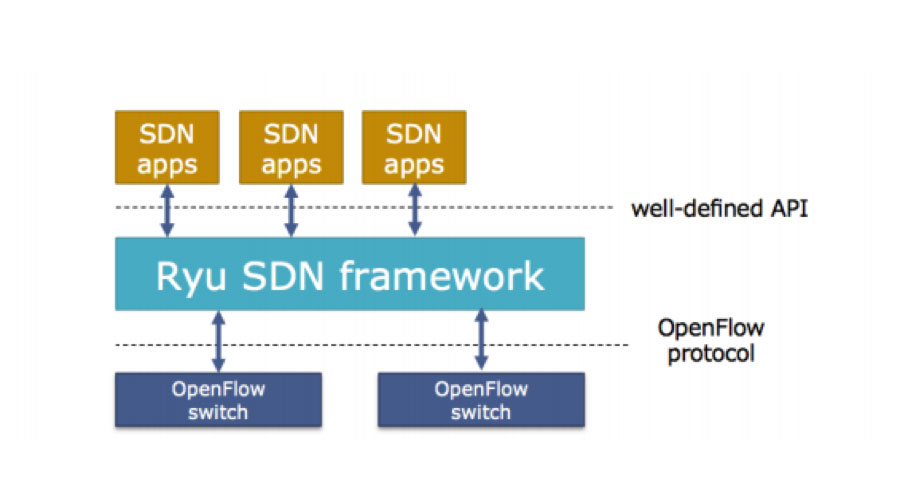
\includegraphics[width=1.0\linewidth]{ryu-controller-sdn-framework}
	  \caption{RYU SDN Controller Framework \cite{ryu_framewrk_png}} \label{fig:ryu-controller-sdn-framework}
	  \vspace{-10pt}
\end{figure}

RYU Controller is supported by NTT of Japan and has a strong open source RYU community that maintain and manage the code which is hosted at GitHub. OpenStack also supports deployment of RYU as network controller in its cloud operating systems.
\subsection{Floodlight Controller \cite{Floodlight_defn}} \label{Floodlight_Controller}

It is yet another open source SDN controller similar to RYU. The benefit of using this controller is the ability to easily develop applications using Java, which is widely used for high level programming by developers and to adapt the software as per requirement. Flood Light offers Representational state transfer application program interface (REST API’s) which help developers to easily program interfaces with the product.

Floodlight is used to run as the network backend for OpenStack. When used with the Neutron plugin with OpenStack, the Floodlight controller functions as a network-as-a-service model with the help of REST API offered by Floodlight. The following diagram below shows the architecture of Floodlight controller.

\begin{figure}[H]
	\centering
	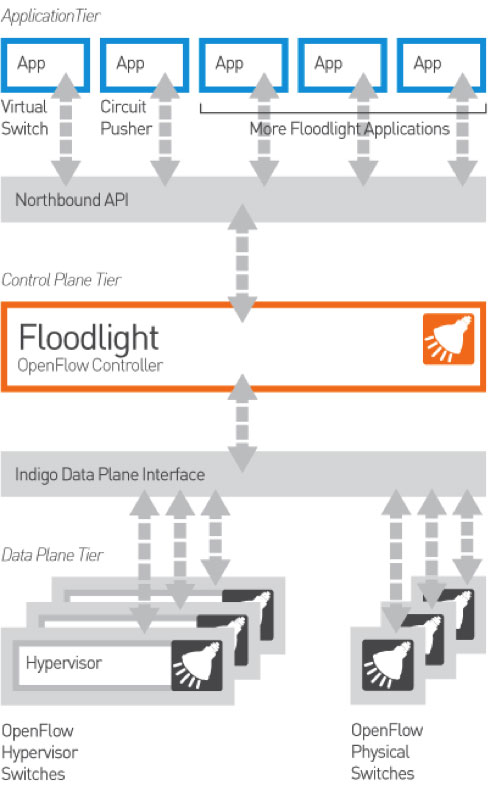
\includegraphics[width=\textwidth, height=\textheight]{floodlight-open-sdn-controller-diagram}
	\caption{Floodlight Controller architecture \cite{Floodlight_arch}} \label{fig:Floodlight_arch}
	\vspace{-10pt}
\end{figure}

\subsection{OpenDaylight} \label{Opendaylight}
OpenDaylight controller is based on JVM, similar to Floodlight, which was a derivative of OpenDaylight that can be deployed on any systems that supports Java. OpenDaylight controller uses the following tools as its framework:

\begin{itemize}
	\item \textbf{Maven:} OpenDaylight uses Maven, which uses Project Object Model to script the dependencies between the bundles for easier build automation.
	\item \textbf{OSGi:} It works as the back-end for OpenDaylight as it loads bundles dynamically and packages JAR files and binding them together for exchange of information.
	\item \textbf{JAVA interfaces:} They are used for event listening, specifications, and forming patterns. 
	\item \textbf{REST APIs:} These are the northbound APIs that manage the topology, flow program, host tracking, static routing and so on.
	
\end{itemize}

The following figure shows the framework of OpenDaylight with the above tools mentioned:

\begin{figure}[H]
	\centering
	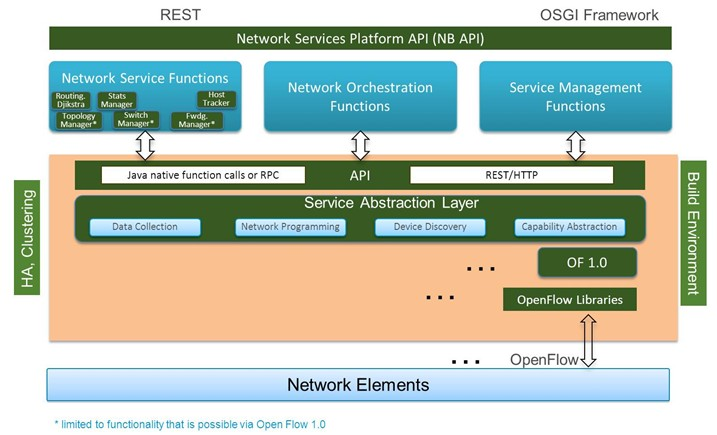
\includegraphics[width=1.0\linewidth]{Architectural_Framework}
	\caption{OpenDaylight Architecture Framework \cite{OpenDaylight_framework}} \label{fig:OpenDaylight_framework}
	\vspace{-10pt}
\end{figure}

\section{Applications of SDN} \label{SDN_applications}

Many research efforts has been done till now in writing SDN applications. Jose et. al. \cite{jose2011online} propose using commodity OpenFlow enabled switches for traffic measurement. The authors propose a framework where a collection of rules are installed on OpenFlow switches, and having a controller track the corresponding flow match counters. The controller can then draw inferences from the counters and dynamically tune the rules as required in order to identify different traffic aggregates.

Resonance \cite{Nayak:2009:RDA:1592681.1592684} is another application uses programmable switches to enforce access control in the network. The authors try to prove that today’s enterprise networks rely on different combinations of middle boxes, intrusion detection systems, and network configurations in order to enforce access control policies, whilst placing a burden on end-hosts in the system to remain patched and secure. The proposed system uses an SDN approach comprising programmable switches and a controller, which together implement a network monitoring framework, a policy specification framework, and the ability to trigger specific actions at the switch level.

OpenSAFE \cite{ballard2010extensible} is a framework that enables network monitoring using OpenFlow. It addresses the problem of routing traffic for network analysis in a reliable manner without affecting normal traffic. 

Hedera \cite{al2010hedera} is an adaptive flow scheduling system for data center networks. The premise for Hedera is that existing IP multipathing techniques used in data centers usually rely on per-flow static hashing, which can lead to under-utilisation of some network paths over time due to hash collisions. The system works by detecting large flows at the edge switches of a data center, and using placement algorithms to find good paths for the flows in the network. Experiments performed using simulations indicate significant improvements over static load balancing techniques. 

In the paper \textit{OpenFlow based server load balancing gone wild} \cite{wang2011openflow}, the authors address the problem of server load balancing using OpenFlow switches. The number of flow entries that can be saved on an OpenFlow switch is much less than the number of unique flows that a switch might need to handle in data center workloads. Thus, micro flow management using per-flow rules is not practical for performing distributing flows between different servers using a switch. The authors thus take advantage of OpenFlow’s wildcard based rules capability, and propose algorithms to compute concise wildcard rules that achieve a specific distribution of traffic.

These are some of the applications that have been written for SDN controllers but none of them address the challenge to dynamically redirect packets in real time, based on different clients and their credentials used for authentication. This thesis proposed to build one such application that can segregate packets coming from different clients in such a way that there is no possible connection between multiple clients associated within the same access point.



%The OpenStack consists of several key service projects which needs to be installed seperately.
%These projects work together depending on the user's cloud needs.
%The projects include Compute, Identity Service, Networking, Image Service, Block Storage, Object Storage, Telemetry, Orchestration, and Database.
%Any services can be installed seperately and configure them stand-alone or as connected entities.
%
%The Liberty version of OpenStack has been installed for the cloud test setup which has been documented in this thesis.
%The OpenStack installation guide can also be found at \href{http://docs.openstack.org/liberty/install-guide-ubuntu/} {OpenStack Installation Guide for Ubuntu}.
%
%The OpenStack project is an open source cloud computing platform that supports all types of cloud environments.
%The project aims for simple implementation, massive scalability, and a rich set of features.
%Cloud computing experts from around the world contribute to the project.
%
%OpenStack provides an Infrastructure-as-a-Service (IaaS) solution through a variety of complemental services.
%Each service offers an application programming interface (API) that facilitates this integration.
%
%
%%\blindtext[1]
%
%\section{Minimum hardware requirements for the compute purpose of the cloud}\label{sec:hardwarerequirements}
%It requires at the least two nodes(hosts) to set up the OpenStack and launch a virtual machine or instance.
%Optional services such as Block Storage and Object Storage require additional nodes.
%
%The hardware architecture explained is the minimal hardware requirements for each type of node.
%The figure \ref{fig:hwreqs} gives a general idea about the required nodes and optional nodes to start with an OpenStack for compute.
%
%\begin{figure}[H]
%  \centering
%  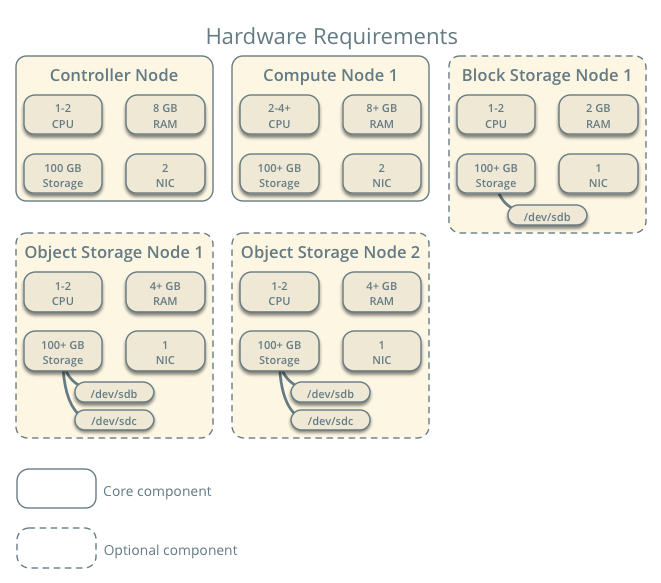
\includegraphics[width=1.0\linewidth]{hwreqs}
%  \caption{Minimum hardware requirements to set up the OpenStack test bed\cite{OpenStack:hwreqs}}\label{fig:hwreqs}
%  \vspace{-10pt}
%\end{figure}
%
%
%\subsection{Controller}\label{ssec:hwcontroller}
%The \verb|controller| node runs the Identity service, Image service, management portions of Compute, management portion of Networking, various Networking agents, and the dashboard. It also includes supporting services such as an SQL database, message queue, and Network Time Protocol.
%
%Optionally, the \verb|controller| node runs portions of Block Storage, Object Storage, Orchestration, and Telemetry services.
%
%The \verb|controller| node requires a minimum of two network interfaces, 8 GB of RAM, 100 GB of storage space.
%
%\subsection{Compute}\label{ssec:hwCompute}
%The \verb|compute| node runs the hypervisor portion of Compute that operates instances.
%By default, Compute uses the KVM hypervisor.
%The \verb|compute| node also runs a Networking service agent that connects instances to virtual networks and provides firewalling services to instances via security groups.
%
%You can deploy more than one \verb|compute| node.
%Each node requires a minimum of two network interfaces,
%more than 8 GB of RAM,
%more than 100 GB of storage space and more than 2 CPU cores.
%
%\subsection{Block Storage}\label{ssec:hwblockstorage}
%This is an optional implementation and has not been set up for the test bed for this thesis.
%The optional Block Storage node contains the disks that the Block Storage service provisions for instances.
%
%You can deploy more than one block storage node.
%Each node requires a minimum of one network interface.
%
%\subsection{Object Storage}\label{ssec:hwobjectstorage}
%This is also an optional implementation and has not been set up for the test bed for this thesis.
%The optional Object Storage node contain the disks that the Object Storage service uses for storing accounts, containers, and objects.
%
%This service requires two nodes.
%Each node requires a minimum of one network interface.
%You can deploy more than two object storage nodes.
%
%\section{Networking Options}\label{sec:Networkingoptions}
%OpenStack provides two diferent networking options:
%\begin{itemize}
%	\item Networking Option 1: Provider networks
%	\\The provider networks option deploys the OpenStack Networking service in the simplest way possible with primarily layer-2 (bridging/switching) services and VLAN segmentation of networks.
%	Essentially, it bridges virtual networks to physical networks and relies on physical network infrastructure for layer-3 (routing) services.
%	Additionally, a DHCP service provides IP address information to instances.
%
%	\item Networking Option 2: Self-service networks
%	\\The self-service networks option augments the provider networks option with layer-3 (routing) services that enable self-service networks using overlay segmentation methods such as VXLAN.
%	Essentially, it routes virtual networks to physical networks using NAT.
%	Additionally, this option provides the foundation for advanced services such as LBaaS and FWaaS.
%\end{itemize}
%
%Considering the network options, the networking option 2 of self service networks have been implemented for the test bed.
%
%%Weiterführende Informationen zu diesem Thema bietet~\cite{Herrmann2004}. In dem Buch werden auch Details zu \acp{ic}
%%dargestellt.
%%\blindtext[2]
%%\blindenumerate{}
%%\blindtext[2]
%
%\section{Configuration of Services and config files}\label{sec:configurationofopenstack}
%
%For the test bed of this thesis, there is one \verb|controller| node and four \verb|compute| nodes which have been configured.
%All the nodes have been installed with the \verb|Ubuntu 14.04| \verb|LTS| Operating system.
%For the purpose of having the GUI, the desktop version of the Operating system has been set up on each node.
%
%This thesis does not explain the installation in detail as it is already available in \href{http://docs.openstack.org/liberty/install-guide-ubuntu/} {OpenStack Installation Guide for Ubuntu}.
%This thesis covers the basics of the topics which were covered during the setup of the test bed are documented. And also, the problems that were faced due to some of the missing configurations as they were not mentioned in the \href{http://docs.openstack.org/liberty/install-guide-ubuntu/} {OpenStack Installation Guide for Ubuntu} are documented in this section.
%
%To keep the configuration of the testbed simple, the password used for convenience on all the host machines and all the OpenStack services is \verb|user|.
%
%
%\subsection{Host networking}\label{ssec:Hostnetworkingarchitecture}
%
%\begin{figure}[H]
%  \centering
%  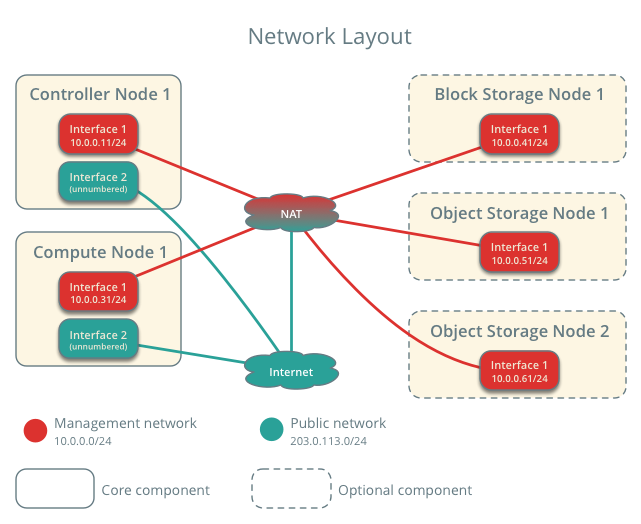
\includegraphics[width=1.0\linewidth]{networklayout}
%  \caption{Network layout among all the host machines\cite{OpenStack:networklayout}}\label{fig:networklayout}
%\end{figure}
%The figure \ref{fig:networklayout} shows how the connections are established between all the node machines.
%A private management network and a public network provided with internet connection are set up for the \verb|controller| and \verb|compute| nodes.
%The management network's IP for the network interface of \verb|controller| node is set to static IP of \verb|10.0.0.11|.
%Similarly, the management network's IP for one of the network interfaces on the five of the \verb|compute| nodes have the static IPs ranging from \verb|10.0.0.31| to \verb|10.0.0.35|.
%
%In this thesis, the storage nodes have not been implemented.
%
%For the testbed setup, one \verb|controller| node and five computes nodes have been set up.
%
%
%\subsection{Network Time Protocol (NTP)}\label{ssec:NetworkTimeProtocol_NTP}
%The Chrony application is installed on all the nodes to synchronise the time on all the installed nodes.
%The \verb|controller| node is set to synchronise with the network time server provided by "TU-Chemnitz" given by the server host name as \verb|ntphost1.hrz.| \verb|tu-chemnitz.de|.
%The other \verb|compute| nodes are set to have the synchronised time with the \verb|controller| node by setting the \verb|controller| node as network time server.
%
%\subsection{OpenStack packages}\label{ssec:OpenStackpackages}
%OpenStack packages are installed on all the nodes by enabling the OpenStack repository and installing all required basic packages.
%
%The MariaDB SQL database server is installed on the \verb|controller| node to store the information related to OpenStack services for authentication and other related activities.
%The MongoDB NoSQL database is installed on the \verb|controller| for the purpose of Telemetry service (Ceilometer).
%
%OpenStack uses the message queue to co-ordinate operations and services among the installed services.
%The RabbitMQ server is installed on the \verb|controller| node to provide the message queue service among the services.
%
%
%\subsection{Add the Identity service}\label{ssec:AddtheIdentityservice}
%The OpenStack Identity service provides a single point of integration for managing authentication, authorization, and service catalog services.
%Other OpenStack services use the Identity service as a common unified API.
%
%When an OpenStack service receives a request from a user, it checks with the Identity service whether the user is authorized to make the request.
%
%In the setup, the Identity service has been installed on the \verb|controller|.
%
%The keystone service entity and API endpoints are created to enable and access the Identity service by internal service calls and from the external requests using the REST based API.
%The public, the internal and the admin endpoints are created to access the Identity service.
%These three endpoints are created across all further services installed.
%
%Each service that you add to your OpenStack environment requires one or more service entities and three API endpoint variants in the Identity service.
%
%While configuring the endpoints for the Identity service, the \verb|region| is set to \verb|TUChem|-\verb|nitz|.
%For example:
%\begin{lstlisting}[frame=single]
%$ openstack endpoint create --region TUChemnitz identity public http://controller:5000/v2.0
%\end{lstlisting}
%
%\comment{A point to remember is, do not duplicate the given endpoints for a given region.
%This has caused the issue with failure of the service.}
%
%Create the projects, users, and roles in the Identity service to access the services for \verb|compute| users for user specific projects based on the access permissions.
%
%The test bed has two projects (admin, demo) for test, 3 diferent users (admin, demo, service) to different access permissions defined by two roles (admin, user).
%
%\subsection{Add the Image service}\label{ssec:AddtheImageservice}
%The OpenStack Image service is central to Infrastructure-as-a-Service (IaaS) as shown in figure \ref{fig:openstack_architecture}.
%It accepts API requests for disk or server images, and image metadata from end users or OpenStack Compute components.
%It also supports the storage of disk or server images on various repository types, including OpenStack Object Storage.
%
%The SQL database is used to store the metadata information of the operating system image or the server image or the disk storage.
%There are templates available of specified requirements to create a virtual machine.
%These templates are called as flavors in OpenStack.
%The details of requirements to boot a virtual machine is defined in these flavors.
%For example, the hard disk capacity, the RAM capacity, the number of virtual cores, which would be required to satisfy the minimum requirements criteria of the desired operating system or to build a robust compute machine with a higher configurations a template is created to give as an input to the scheduler to create a virtual machine.
%
%This service is installed on \verb|controller| node.
%The glance service entity and the API endpoints are created.
%While configuring the endpoints for the Image service, the \verb|region| is set to \verb|TUChemnitz|.
%For example:
%\begin{lstlisting}[frame=single]
%$ openstack endpoint create --region TUChemnitz image public http://controller:9292
%\end{lstlisting}
%
%The \verb|cirros-0.3.4-x86_64-disk.img| disk image was downloaded and added to the image service as a bootable image of Cirros operating system to create and boot virtual machines.
%
%
%\subsection{Add the Compute service}\label{ssec:AddtheComputeservice}
%OpenStack Compute is a major part of an Infrastructure-as-a-Service (IaaS) system.
%The main modules are implemented in Python.
%
%OpenStack Compute interacts with OpenStack Identity for authentication, OpenStack Image service for disk and server images, and OpenStack dashboard for the user and administrative interface. Image access is limited by projects, and by users; quotas are limited per project (the number of instances, for example). OpenStack Compute can scale horizontally on standard hardware, and download images to launch instances.
%
%The nova service entity and the API endpoints are created.
%While configuring the endpoints for the Compute service, the \verb|region| is set to \verb|TUChemnitz|.
%For example:
%\begin{lstlisting}[frame=single]
%$ openstack endpoint create --region TUChemnitz compute public http://controller:8774/v2/%\(tenant_id\)s
%\end{lstlisting}
%
%RabbitMQ which is the installed message queue server is used to pass the communication messages between the nodes and the other services.
%The MariaDB SQL database stores the build-time and run-time states of the whole cloud infrastructure like available instance, instances in use, available networks and different projects.
%
%The OpenStack compute is installed with required packages on \verb|controller| node which are different than the \verb|compute| node.
%The important compute services like \texttt{nova-scheduler, nova-conductor, nova-api, nova-cert, nova-novncproxy} and \texttt{python-novaclient} are installed on the \verb|controller| node.
%The configuration of RabbitMQ message service needs some additional parameters that needs to be added in the \verb|/etc/nova/nova.conf| configuration file in the \verb|controller| node under the \verb|[oslo_messaging_rabbit]|.
%
%\begin{lstlisting}[frame=single]
%[oslo_messaging_rabbit]
%rabbit_host = controller
%rabbit_port = 5672 #define ports
%rabbit_hosts = controller:5672
%rabbit_userid = openstack
%rabbit_password = user
%rabbit_use_ssl = false
%\end{lstlisting}
%
%\comment{The compute service failed to function when the \texttt{rabbit\_port} was not defined in the configuration.}
%
%The OpenStack compute is installed with the \verb|nova-compute| package on all the \verb|compute| nodes.
%The configuration of RabbitMQ message service needs some additional parameters that needs to be added in the \verb|/etc/nova/nova.conf| configuration file in the \verb|compute| nodes under the \verb|[oslo_messaging_rabbit]|.
%\\Please refer to Appendix \nameref{app:sec:rabbitmq_config} for the \verb|[oslo_messaging_rabbit]| configuration parameters.
%
%%\begin{lstlisting}[frame=single]
%%[oslo_messaging_rabbit]
%%rabbit_host = controller
%%rabbit_port = 5672 #define ports
%%rabbit_hosts = controller:5672
%%rabbit_userid = openstack
%%rabbit_password = user
%%rabbit_use_ssl = false
%%\end{lstlisting}
%
%In the \texttt{[DEFAULT]} section of the \verb|/etc/nova/nova.conf| file in \verb|compute| nodes, configure the \verb|my_ip| option with their respective management IP address of the compute nodes.
%
%In the \texttt{[vnc]} section of the \verb|/etc/nova/nova.conf| file in \verb|compute| nodes, enable and configure remote console access by providing the public base url of the \verb|controller| node to make it accessible from any machine outside the management network.
%
%\begin{lstlisting}[frame=single]
%[vnc]
%enabled = True
%vncserver_listen = 0.0.0.0
%vncserver_proxyclient_address = $my_ip
%novncproxy_base_url = http://os-controller.etit.tu-chemnitz.de:6080/vnc_auto.html
%\end{lstlisting}
%
%Verify the operation of the Compute service by performing the commands as stated in the \href{http://docs.openstack.org/liberty/install-guide-ubuntu/} {OpenStack Installation Guide for Ubuntu}.
%
%\subsection{Add the Networking service}\label{ssec:AddtheNetworkingservice}
%This section explains about installation and configuration of the OpenStack Networking service (neutron) using the \verb|self-service networks| option.
%OpenStack Networking (neutron) allows you to create and attach interface devices managed by other OpenStack services to networks.
%
%OpenStack Networking (neutron) manages all networking facets for the Virtual Networking Infrastructure (VNI) and the access layer aspects of the Physical Networking Infrastructure (PNI) in any given OpenStack environment.
%OpenStack Networking enables tenants to create advanced virtual network topologies which may include services such as a firewall, a load balancer, and a virtual private network (VPN).
%
%Networking provides networks, subnets, and routers as object abstractions.
%
%The neutron service entity and the API endpoints are created.
%While configuring the endpoints for the Networking service, the \verb|region| is set to \verb|TUChemnitz|.
%For example:
%\begin{lstlisting}[frame=single]
%$ openstack endpoint create --region TUChemnitz network public http://controller:9696
%\end{lstlisting}
%The Networking option 2: Self service networks is adapted for configuration of the test bed.
%
%The required neutron networking components are installed on the \verb|controller| node.
%The configuration of RabbitMQ message service needs some additional parameters that needs to be added in the \verb|/etc/neutron/neutron.conf| configuration file in the \verb|controller| node under the \verb|[oslo_messaging_rabbit]|.
%\\Please refer to Appendix \nameref{app:sec:rabbitmq_config} for the \verb|[oslo_messaging_rabbit]| configuration parameters.
%
%%\begin{lstlisting}[frame=single]
%%[oslo_messaging_rabbit]
%%rabbit_host = controller
%%rabbit_port = 5672 #define ports
%%rabbit_hosts = controller:5672
%%rabbit_userid = openstack
%%rabbit_password = user
%%rabbit_use_ssl = false
%%\end{lstlisting}
%
%In the \verb|/etc/neutron/neutron.conf| configuration file of the controller, under the \verb|[nova]| section, the \verb|region_name| is set to \verb|TUChemnitz|.
%\begin{lstlisting}[frame=single]
%[nova]
%...
%region_name = TUChemnitz
%\end{lstlisting}
%
%In the \verb|/etc/neutron/metadata_agent.ini| file of the controller, under the \verb|[DEFAULT]| section, the \verb|auth_region| is set to \verb|TUChemnitz|.
%The \verb|metadata_proxy_shared_-| \verb|secret| is set to \verb|user| which will be used in \verb|/etc/nova/nova.conf| configuration file.
%\begin{lstlisting}[frame=single]
%[DEFAULT]
%...
%auth_region = TUChemnitz
%...
%metadata_proxy_shared_secret = user
%\end{lstlisting}
%
%Edit the \verb|/etc/nova/nova.conf| configuration file to set the \verb|metadata_proxy_share|-\verb|d_secret| with the value of \verb|user|.
%\begin{lstlisting}[frame=single]
%[neutron]
%...
%region_name = TUChemnitz
%...
%metadata_proxy_shared_secret = user
%\end{lstlisting}
%
%Once the \verb|controller| node has been set up, the common Networking components are installed on each of the \verb|compute| nodes.
%The configuration of RabbitMQ message service needs some additional parameters that needs to be added in the \verb|/etc/neutron/n|-\verb|eutron.conf| configuration file in each of the \verb|compute| node under the \verb|[oslo_messag|-\verb|ing_rabbit]|.
%\\Please refer to Appendix \nameref{app:sec:rabbitmq_config} for the \verb|[oslo_messaging_rabbit]| configuration parameters.
%
%%\begin{lstlisting}[frame=single]
%%[oslo_messaging_rabbit]
%%rabbit_host = controller
%%rabbit_port = 5672 #define ports
%%rabbit_hosts = controller:5672
%%rabbit_userid = openstack
%%rabbit_password = user
%%rabbit_use_ssl = false
%%\end{lstlisting}
%
%As the \textit{Networking option 2: Self service networks} was set up in \verb|controller| node, the Linux bridge agent, which builds layer-2 (bridging and switching) virtual networking infrastructure for instances including VXLAN tunnels for private networks and handles security groups, is configured on each \verb|compute| node.
%
%As in \verb|controller| node, the \verb|compute| nodes are configured to use the networking service by editing the \verb|/etc/nova/nova.conf| configuration file on each \verb|compute| node.
%\begin{lstlisting}[frame=single]
%[neutron]
%...
%region_name = TUChemnitz
%\end{lstlisting}
%
%The configuration of networking service is verified to have all the services of networking to be active.
%
%\subsection{Add the dashboard}\label{ssec:Addthedashboard}
%The OpenStack Dashboard, also known as horizon is a web interface that enables cloud administrators and users to manage various OpenStack resources and services.
%
%The Dashboard enables web-based interactions with the OpenStack Compute cloud controller through the OpenStack APIs.
%
%Horizon enables you to customize the brand of the dashboard.
%
%The dashboard relies on functional core services including identity, image, compute, and neutron.
%The dashboard is installed on the \verb|controller| node.
%
%The figure \ref{fig:dashboard_login} shows the login screen for the OpenStack dashboard.
%
%\begin{figure}[H]
%  \centering
%  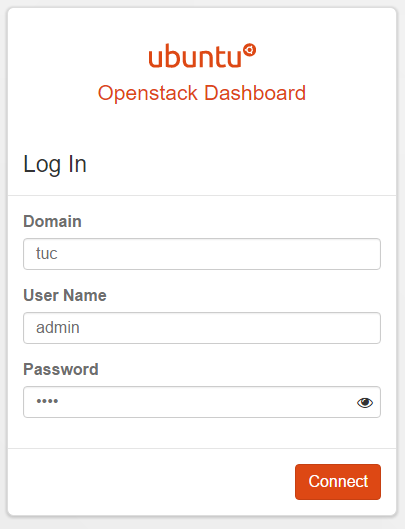
\includegraphics[width=0.7\linewidth]{dashboard_login}
%  \caption{Login screen for the dashboard}\label{fig:dashboard_login}
%\end{figure}
%The dashboard can be accessed by using the web browser at: \\\verb|http://os-controller.etit.tu-chemnitz.de/horizon|.
%
%Provide the login credentials to authenticate the user against the Keystone to login into the Dashboard.\\
%
%The login credentials are:
%\\Domain: \verb|TUC|
%\\User Name: \verb|admin| or \verb|demo|
%\\Password: user
%
%The figure \ref{fig:network_topology_dashboard_view} shows the pictorial representation of the network and the instances created on the OpenStack under the link \textit{Network Topology}.
%
%\begin{figure}[H]
%  \centering
%  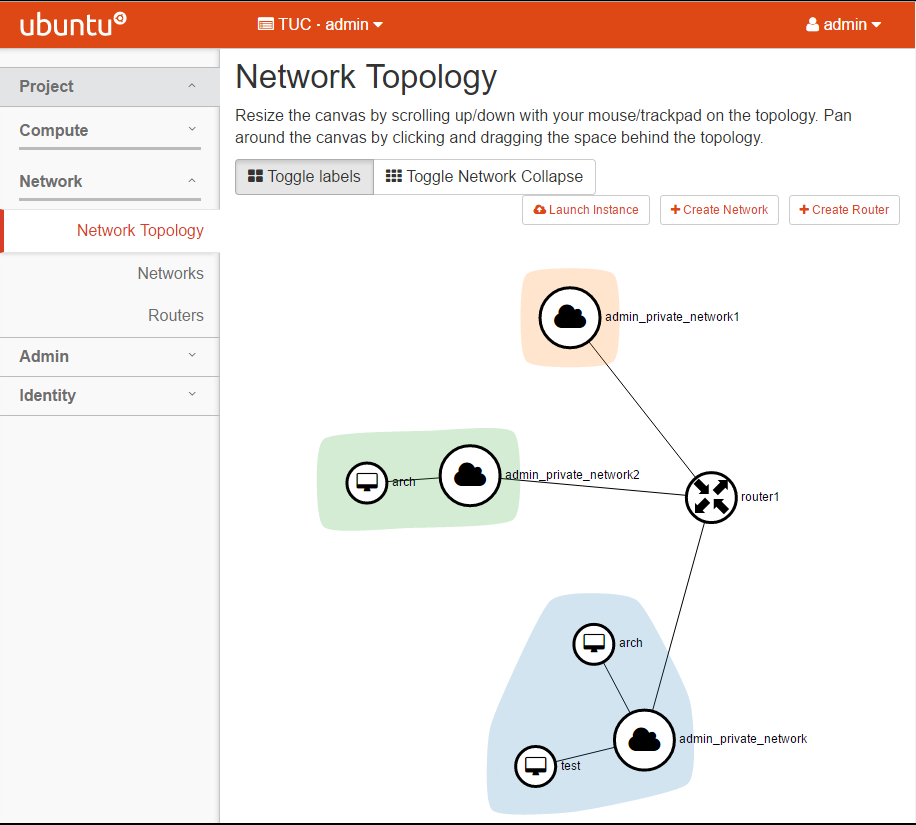
\includegraphics[width=1.0\linewidth]{network_topology_dashboard_view}
%  \caption{The dashboard screen showing the diagrammatic representation of network topology}\label{fig:network_topology_dashboard_view}
%\end{figure}
%
%\subsection{Add the Telemetry service}\label{ssec:AddtheTelemetryservice}
%The Object storage and Bloack storage services have not been deployed for the test bed.
%The next service deployed is the OpenStack Telemetry service.
%
%Telemetry service is deployed to have an analysis of metering data with respect to Compute and Image services.
%Telemetry helps to efficiently poll the metering data related to OpenStack services.
%
%Unlike other services, the Telemetry service uses a NoSQL database.
%The MongoDB NoSQL server has been installed on the controller to be utilised by the Telemetry service.
%The \verb|password| for the MongoDB is set to \verb|user|.
%
%The ceilometer service entity and the API endpoints are created.
%While configuring the endpoints for the Telemetry service, the \verb|region| is set to \verb|TUChemnitz|.
%For example:
%\begin{lstlisting}[frame=single]
%$ openstack endpoint create --region TUChemnitz metering public http://controller:8777
%\end{lstlisting}
%
%
%The configuration of RabbitMQ message service needs some additional parameters that needs to be added in the \verb|/etc/ceilometer/ceilometer.conf| configuration file on the \verb|controller| node under the \verb|[oslo_messaging_rabbit]|.
%\\Please refer to Appendix \nameref{app:sec:rabbitmq_config} for the \verb|[oslo_messaging_rabbit]| configuration parameters.
%%\begin{lstlisting}[frame=single]
%%[oslo_messaging_rabbit]
%%rabbit_host = controller
%%rabbit_port = 5672 #define ports
%%rabbit_hosts = controller:5672
%%rabbit_userid = openstack
%%rabbit_password = user
%%rabbit_use_ssl = false
%%\end{lstlisting}
%
%In the \verb|[service_credentials]| section, the \verb|os_region_name| is set as \verb|TUChemnitz|.
%\begin{lstlisting}[frame=single]
%[service_credentials]
%...
%os_region_name = TUChemnitz
%\end{lstlisting}
%
%Once the Telemetry service has been installed on \verb|controller|, it is configured to be consumed by Image service by editing the existing \verb|/etc/glance/glance-api.conf| and \verb|/etc/glance/glance-registry.conf| configuration files by adding the \\\verb|[oslo_messaging_rabbit]|.
%\\Please refer to Appendix \nameref{app:sec:rabbitmq_config} for the \verb|[oslo_messaging_rabbit]| configuration parameters.
%
%%\begin{lstlisting}[frame=single]
%%[oslo_messaging_rabbit]
%%rabbit_host = controller
%%rabbit_port = 5672 #define ports
%%rabbit_hosts = controller:5672
%%rabbit_userid = openstack
%%rabbit_password = user
%%rabbit_use_ssl = false
%%\end{lstlisting}
%
%Once the OpenStack installation procedure with additional configuration as mentioned above is configured, the Telemetry is for Image service.
%
%To enable the Telemetry service for Compute service, the ceilometer should be installed on each \verb|compute| node.
%Once the Telemetry service has been installed on all the \verb|compute| nodes, it is configured to enable ceilometer by editing the \verb|/etc/ceilometer|-\verb|/ceilometer.conf| configuration file by adding the \verb|[oslo_messaging_rabbit]|.
%Please refer to Appendix \nameref{app:sec:rabbitmq_config} for the \verb|[oslo_messaging_rabbit]| configuration parameters.
%
%%\begin{lstlisting}[frame=single]
%%[oslo_messaging_rabbit]
%%rabbit_host = controller
%%rabbit_port = 5672 #define ports
%%rabbit_hosts = controller:5672
%%rabbit_userid = openstack
%%rabbit_password = user
%%rabbit_use_ssl = false
%%\end{lstlisting}
%
%In the \verb|[service_credentials]| section, the \verb|os_region_name| is set as \verb|TUChemnitz|.
%\begin{lstlisting}[frame=single]
%[service_credentials]
%...
%os_region_name = TUChemnitz
%\end{lstlisting}
%
%
%\begin{figure}[H]
%  \centering
%  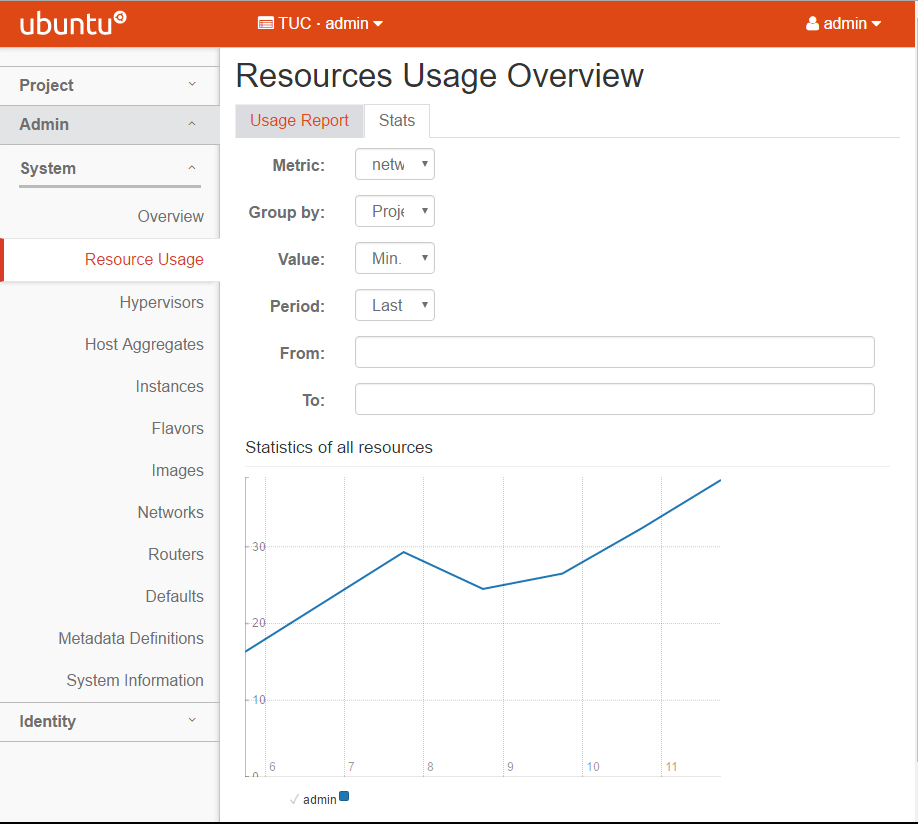
\includegraphics[width=1.0\linewidth]{telemetry_network_incoming_bytes}
%  \caption{An example of the metering with the number of incoming bytes on a network for a virtual machine interface.}\label{fig:telemetry_network_incoming_bytes}
%\end{figure}
%
%All the above mentioned services have been installed and configured in the OpenStack test bed for this thesis.

%Das hier vorgestellte basiert auch dem Buch von~\cite{Heinkel2000}. Die Lösung kann auch mit einem \ac{fpga} sowie
%\ac{hw} und \ac{sw} entstehen.
%\blindtext[4]

%\subsection{Zweite Untergrundlage}\label{ssec:zweiteUGdl}

%\blindtext[1]
%\begin{table}[htpb]
%  \centering
%  \caption{Eine tolle Tabelle}\label{tab:ett}
%  \begin{tabular}{lcrl}
%  Links & Zentriert & Rechts & Links \\
%  \toprule
%  eins & zwei & drei & vier \\
%  eins & zwei & drei & vier \\
%  eins & zwei & drei & vier \\
%  \end{tabular}
%\end{table}

%Eine Tabelle benötigt auch eine Referenz, wie diese hier zu \ref{tab:ett}.
%\blindtext[1]

%\section{Zweite Grundlage}\label{sec:zweitegdl}

%\blindtext[2]

%\section{Dritte Grundlage}\label{sec:drittegdl}

%\blindtext[2]

% vim: ts=2:sw=2:sts=2:expandtab:wrapmargin=2:tw=120

